% \setchapterstyle{kao}
\setchapterimage[6.5cm]{internet_03}
\setchapterpreamble[u]{\margintoc}
\chapter[智能家居与互联网]{智能家居与互联网\footnotemark[0]}

\footnotetext{The credits for the image above the chapter title go to:
	Image generated by OpenAI's DALL-E, used in accordance with OpenAI's terms and conditions.}


\section{前言}

不知不觉间,人工智能已经渗透到我们生活的每个角落。回到家中,有人工智能的“仆人”智能家居给我们提供便捷舒适的服务,打开手机,一键开启家中的灯光,打开窗帘,空调也自动调整到了舒适的温度。坐在沙发上,打开手机刷刷短视频,抖音已经用人工智能技术给我们规划好的今天要推送的视频,突然刷到了一个商品的推荐广告视频,你觉得很感兴趣,于是打开淘宝,发现你想要的商品已经出现在了商品栏的第一列,商品的描述写的很有文采,像一首诗一样押韵,你有点感叹商家不仅要学习怎么售卖商品,还要具备这么高的文学素养了,丝毫没有怀疑这些诗一般的商品描述其实是人工智能根据商品的简单描述生成出来的风格化文本。

在这一章节,首先我们将介绍搜索引擎和推荐系统。对于推荐算法,经常看短视频或者网购的人应该都不会陌生,但你是否曾经会产生疑问:在当前人人都能发视频的年代,每天更新的视频可能有百万的数量级,如此庞大的视频海洋中,人工智能又是如何精确发现每个用户喜欢的视频的呢?难道是把所有视频都查看一遍,然后选出最高相关度的视频吗?显然当前的硬件算力还不足以支持如此低效的算法,要是有1万个用户,那么1万个视频就要计算1万乘1万次相关度,也就是1亿次计算开销,更何况一个较为热门的视频平台,如抖音,bilibili上,用户都是千万起步的,如此庞大的计算开销是不可能实现的。人工智能技术则能让推荐系统以较低的开销实现快速的定位相关视频并推荐给用户,如此神奇的技术的原理将在第一小节揭晓。

在第二章节,我们将介绍当前智慧客服的原理。对于经常使用在线客服服务的人来说,智能客服已经成为了生活中不可或缺的一部分。然而,你是否曾想过,智能客服是如何在短时间内理解用户的问题,并提供恰当的回答的呢?难道是人工客服在后台实时回应吗?显然,这种方式在效率和成本上都无法满足大规模服务的需求。人工智能技术在这里发挥了关键作用。通过使用自然语言处理和机器学习技术,智能客服系统能够自动处理大量常见的用户问题,提供实时支持,从而大大提高了客户满意度和服务效率。此外,智能客服系统还能够不断学习和优化,以提高自身的回答准确性和适应性,为用户提供更加个性化的服务。

在第三章节,我们将深入探讨人工智能在智能家居中的运用。或许很多人都没有意识到,AI这个无形的东西已经悄无声息地融入我们的日常生活,为我们带来了很多的便捷和好处。在智能家居中,人工智能可以结合物联网技术,学习到每个用户的作息时间、生活习惯以及健康状态等信息。基于这些数据,智能家居系统能够为我们规划好生活中的琐事,如自动调节室内温度、灯光和通风等,让我们能够享受到更加舒适的生活环境。此外,智能家居系统还能根据用户的用电习惯和设备使用情况,为我们规划电器的电量消耗,从而达到节能的目的。通过优化家电的运行模式,智能家居系统能够帮助我们节省电费,减少能源消耗,实现绿色环保的生活理念。在这一章节中,我们将详细介绍人工智能在智能家居中的各种应用场景,以及它是如何通过学习用户行为,为我们的生活带来诸多便利。同时,我们还将探讨智能家居技术在未来的发展趋势,以及它将如何进一步改善我们的生活质量。通过了解智能家居系统的原理,你将能够更好地把握这个正在改变我们生活方式的重要技术。

在第四章节,我们会探讨一个近年来十分火爆的AI创作的原理。AI写诗,AI绘画,AI作曲,都是近年来广受人们欢迎,却又备受争论的话题。当前在网络上,或多或少都会看到一些AI创作的内容,因为AI创作的入门门槛很低,每个人都可以操控AI来创作自己喜欢的作品。只需要简单的输入一个文本提示(prompt),就可以得到相应的画作/诗歌/音乐。通过了解AI创作的原理,你将能够更好地把握这个正在改变艺术世界的重要技术,为未来的创意产业发展做好准备。

在本章节的最后,我们将深入探讨人工智能在网络安全方面的应用,展示其在保护个人隐私和财产安全方面的巨大潜力。在当前数字化时代,网络安全问题日益严峻,恶意代码和钓鱼网站层出不穷,给用户带来了极大的困扰。而人工智能技术正是解决这些问题的关键。通过运用深度学习、自然语言处理等技术,人工智能能够自动识别恶意代码和钓鱼网站,实时保护用户的安全。在本章节中,我们将详细介绍人工智能在网络安全方面的应用原理,以及如何利用这些技术保护个人隐私和财产安全。

\section[搜索引擎与推荐系统]{搜索引擎与推荐系统:AI如何精准导航信息海洋}

\subsection{搜索引擎}
搜索引擎,简而言之,就是帮助查找与搜索相关结果的在线工具。百度搜索和谷歌搜索都是比较广为人知的搜索引擎。它们都需要在信息量庞大的互联网中,通过使用用户输入的简单的字词,找到与之最相关的页面。

随着互联网信息量的不断增长,搜索引擎也需要不断地与时俱进。相比于十几年前的搜索引擎,现在的搜索引擎融合了更多的AI技术如机器学习,深度学习等方法,能更加精准并快速地定位用户搜索的页面。

输入相同的查询词句到不同的搜索引擎中或许会得到不同的结果,但是搜索引擎的工作流程大部分都是大同小异。传统的搜索引擎的工作原理可以大概分为下面的六步:

1. 网页爬取:首先搜索引擎使用爬虫程序搜索并收集互联网上的网页信息。
2. 建立数据库:通过爬虫程序搜集得到的网页会存放在一个数据库中。
3. 网页处理:搜索引擎对数据库中的网页进行预处理,如提取网页中的文本和图片等。
4. 建立索引:搜索引擎根据网页的文本等信息建立相对应的索引。
5. 检索服务:当用户输入关键词时,搜索引擎的检索器会在索引库中快速检索网页,并计算网页与查询关键词的相关度。
6. 结果展现:根据网页与查询关键词的相关度,搜索引擎对根据索引检索到的网页进行排序,并按顺序将网页展现给用户。

通常人工智能技术可以运用于检索服务和结果展现中,为用户提供更加精准且个性化的查询结果。当用户输入查询词句时,搜索引擎就可以使用人工智能中的自然语言处理技术来处理输入的查询词句,例如通过自然语言处理中的实体识别和关系抽取方法来识别出查询中的实体和关键信息,并通过语言模型来分析出其中的语义信息,这样搜索引擎就可以更好地理解用户的查询意图,从而提供给用户更加精准的查询结果。除此之外,如今大部分流行的搜索引擎如百度和谷歌都支持图像检索,当用户输入图像进行查询时,搜索引擎可以使用人工智能中的计算机视觉识别技术来对图像中的人物,场景进行识别,从而实现基于图像的搜索;更进一步地,人工智能可以根据图像输出图像的文本描述,通过该图像的文本描述,搜索引擎可以更准确搜索到用户需要的结果。在结果展现时,搜索引擎可以收集用户的个性化信息和搜索行为,使用机器学习学习算法或者深度学习模型,对用户的偏好进行分析,对搜索结果进行个性化进行排序,提供更为个性化的搜索结果。

在当前大语言模型如ChatGPT,GPT-4大火的时代,很多互联网公司如谷歌和微软亦推出了它们的交互式的搜索引擎。利用大语言模型强大的语言理解能力和交互能力,搜索引擎可以通过多次和用户的交互来逐步构建用户的需求框架,从而为用户提供更符合其需求的结果。
此外,人工智能技术还可以用于优化搜索引擎的广告推送服务。大部分市面上的搜索引擎对于普通的用户来说都是免费的,它们的主要盈利方式就是广告收入。因此广告的点击率决定着这些互联网公司在搜索引擎上能够获得多少的利润。在人工智能大火的时代,他们当然会想方设法地去利用人工智能技术来优化自己的广告推送从而让更多的商家愿意选择在自己的平台上进行广告宣传。具体地,搜索引擎可以利用深度学习模型,通过分析用户的历史搜索记录和网页浏览行为,为用户展示与其搜索意图相关的广告,从而提高广告的点击率。当用户搜索“如何穿搭更为潮流”,搜索引擎就会收集用户的个人信息如年龄性别,还有用户的网页浏览记录,把这些信息全都输入到深度神经网络模型中,就能分析得到更适合用户的服装店的广告。用户看到较为适合自己的服装便会点击进去,广告的点击率也就提升了,自然而然的互联网公司在搜索引擎上获得的利润也就提高了。

\subsection{推荐系统}
互联网的发展带动了电商平台的飞速发展。如今每个人都手机里几乎都有淘宝或者京东这些电商app,如此以来,这些电商平台能获得的客户数据也正以前所未有的速度增长着。人工智能技术成为了有效利用这些数据来个性化用户体验的不二之选。基于机器学习方法的推荐系统可以有效地利用客户数据来个性化用户体验,提高参与度和保留率,并最终推动更大的销售。例如,在2021年,Netfilx公司报道称,其推荐系统每年帮助增加 1 亿美元的收入。 亚马逊是另一家通过向客户提供个性化推荐而受益的公司。 2021年, 亚马逊公司报道称,其推荐系统帮助销售额增加了 35\%。下面我们将更具体地探讨推荐系统。

\begin{marginfigure}
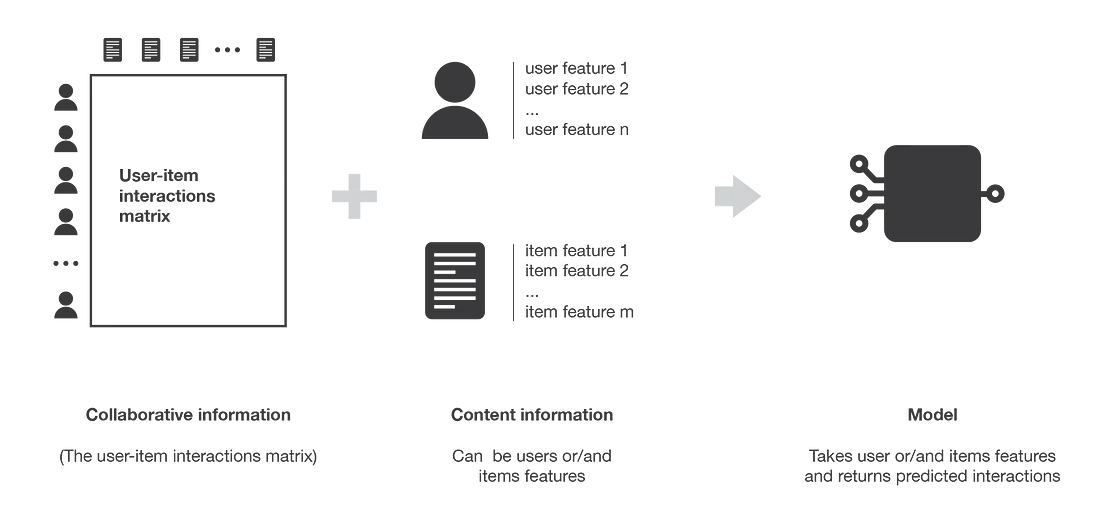
\includegraphics{images/Internet_05.jpg}
\end{marginfigure}

简而言之,推荐系统就是一种使用数据分析和机器学习技术向用户推荐他们可能感兴趣的相关信息(电影、视频、物品)的算法。推荐系统常用的算法主要包括协同过滤,聚类和深度学习等。其中协同过滤是打造个性化推荐时的常用算法,可以分析出与用户有相似兴趣的群体,从而推荐该群体感兴趣的商品给客户。而聚类算法是将未知对象进行归类的算法,在构建智能推荐系统时,若缺失此前用户数据,可选用聚类算法。深度学习算法则是使用深度神经网络分析用户数据来输出用户感兴趣的商品。

实际上,推荐系统并不只是在电商平台上才有应用。社交软件如微信,陌陌,可以根据用户的好友关系和互动记录,推荐给用户新的朋友和内容。视频平台,如哔哩哔哩,抖音等,可以根据用户观看和点赞过的视频来推荐更多相关的视频内容,每次拉下屏幕刷新都是平台的推荐系统计算分析出的用户最可能感兴趣的视频。还有音乐平台,如网易云音乐和QQ音乐,打开每日推荐或是私人漫游,便是推荐系统根据用户听过的歌的风格来给用户量身定制的音乐节目单。

推荐系统让我们每个人都能享受个性化的定制服务,这时也有人会提出担忧“人工智能是不是给每个人都打造了一个信息茧房,所有人会都被困在里面一辈子”。这一点是不可否认的,推荐系统在给每个人个性化的推荐的同时,也变相地限制了每个人能获得的信息,我们很难得到和我们平时所处圈子外的信息,因为推荐系统会认为那些信息都是用户不会感兴趣的,也就不会推送到用户面前。但实际上,相比于人工智能大火前,我们每个人能获取到信息的渠道都十分的有限,在那时候,我们又何尝不是处在一个信息茧房中呢?在人短短的一生中,或许我们能在此信息茧房中得到的信息已经远远超于没有互联网的时代。更进一步地说,信息爆炸的时代,或许是这些基于人工智能技术的推荐系统才让我们免于淹没在信息的海洋中,获得属于我们自己个人的舒适圈吧。

\section[智慧客服]{智慧客服:AI为用户答疑解惑}

\begin{marginfigure}
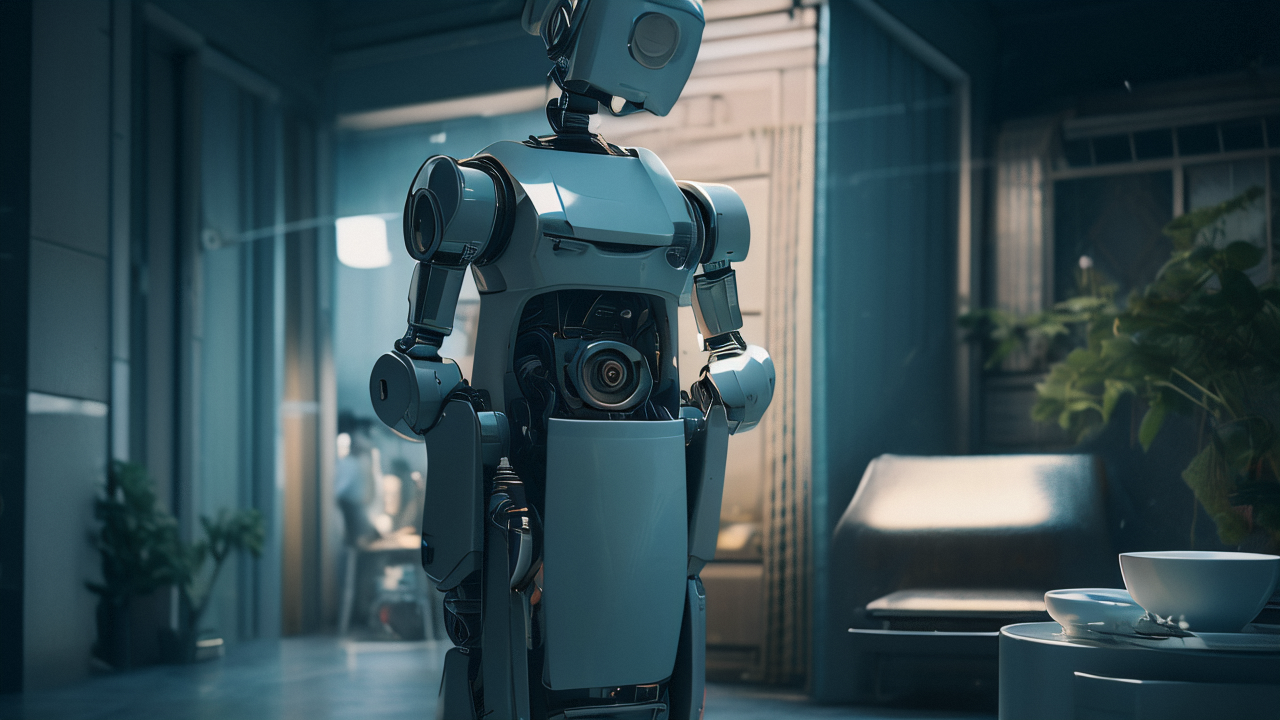
\includegraphics{images/Internet_07.png}
\end{marginfigure}

有一天,你突然接到一个电话,对面自称是某公司的客服,向你调查产品使用体验。如果你配合客服的请求,继续跟他对话,你一点也不会怀疑他是不是真人,因为他能很从容地和你进行交谈,逻辑也毫无漏洞。但是如果你突发奇想,问他一句“你是真人吗”,他或许就会立即宕机,陷入沉默。现在的智慧客服已经不再像过去只能让用户按0或1回答,而是能轻松处理语音文本,并且生成文本,转换为语音来进行对话,然而对于一些刁难的问题,智慧客服却仍然不能很好地处理。那么这样的人工智能的智慧客服是如何进行流畅的对答,又是为何无法回答一些问题的呢?

使用人工智能技术的智慧客服的原理实际上和手机中自带的语音助手类似,它们的整个工作流程都可以分为三步:自动语音识别(ASR),自然语言理解(NLU),语音合成(TTS)。

\section[智能家居与物联网]{智能家居与物联网:AI让生活更智能}

\begin{marginfigure}
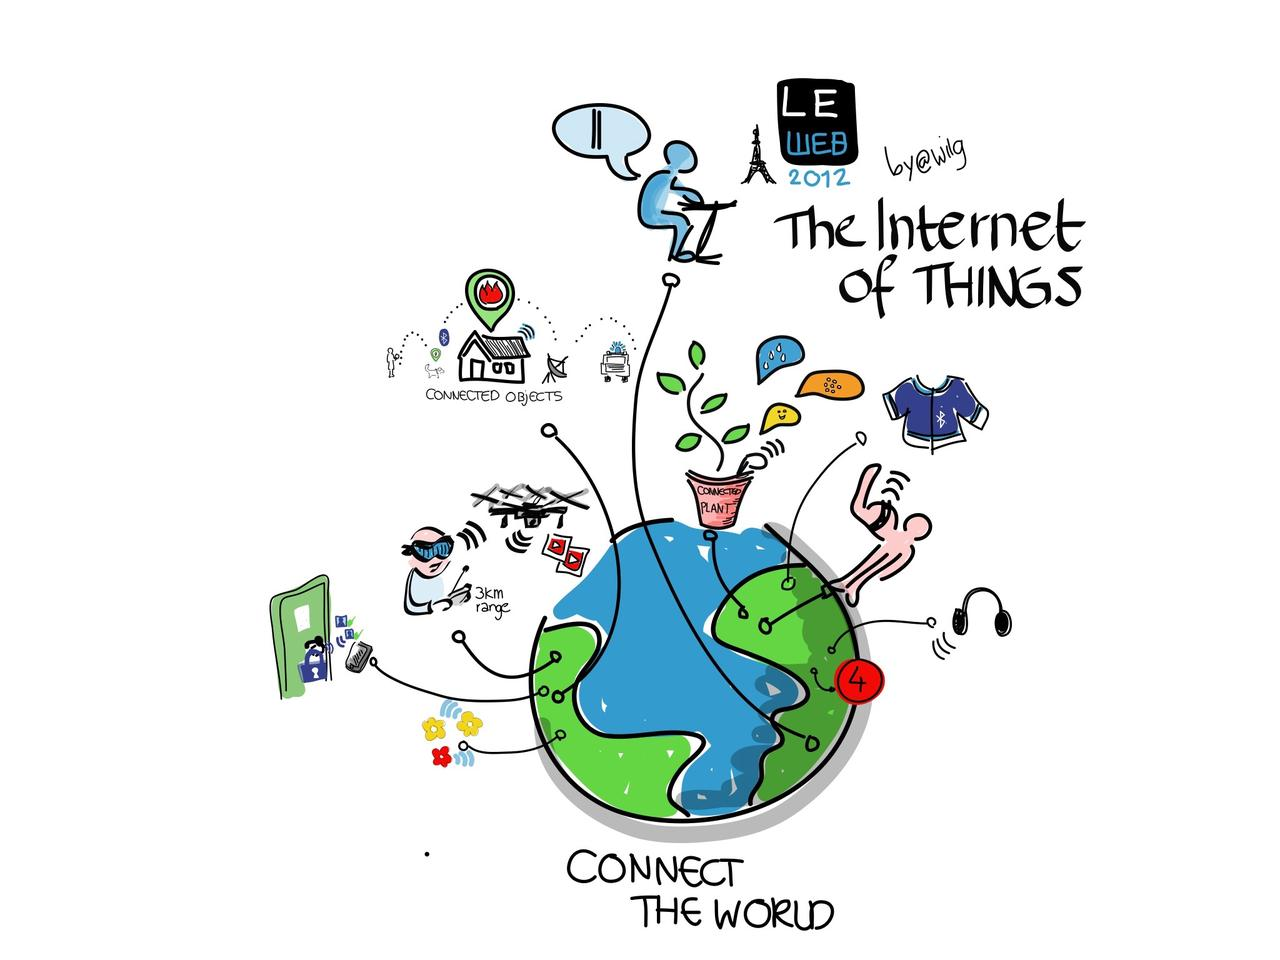
\includegraphics{images/Internet_08.jpg}
\end{marginfigure}

一个炎热的夏天,你工作了一天,拖着疲惫的身体在回家的路上,尽管已经是夜晚了,但白天的余热仿佛仍从地面不断传出来。你打开手机,发现手机上出现了一个提示,询问是否需要开启家中的空调。你毫不犹豫的点击了“是”。一踏入家中,清凉的空调风吹出来,你马上感觉浑身清爽了许多,与此同时,家中的灯也自动打开了,音响也在播放着你最近在音乐软件上收藏的音乐,家里的冷清感立马少了许多。一切都是那么的智能,仿佛有一个专属于你的仆人在家中等着你回家。如此智能的生活便是得益于当前智能家居的广泛使用了。在这小节,我们将探讨AI技术是如何让生活更加的智能和便捷的。

智能家居是指通过先进的信息技术、通信技术和自动化控制技术,将家庭内的各种设备、设施和系统互联互通,实现家庭管理、设备控制、能源管理、安全监控等功能,提高生活品质和便捷性的系统。其原理基于物联网、人工智能、传感器技术等多种技术的综合应用。这些技术的综合应用,使得家庭内的各种设备能够相互配合,实现更加智能化和自动化的控制,从而让我们的生活更加便捷和舒适。

智能家居系统主要可以包含以下几个部分:
1. 家庭网络:为智能家居设备提供网络连接和数据传输通道。
2. 智能设备:如智能照明,智能安防,智能家电等,负责数据采集,处理和执行。
3. 控制中心:作为智能家居系统的核心,负责设备控制,数据分析和决策制定。
4. 用户界面:为用户提供直观,便捷的操作界面,如手机APP,触控面板。
        智能家居的整体工作流程可以总结为:1. 传感器等物理设备收集家中的现实物理信息,并上传到物联网上。2. 物联网整合所有的传感器信息,通过控制中心进行数据分析和决策制定。3. 最终在手机APP上呈现给用户,让用户选择操作。

\subsection{物联网技术在智能家居中的应用}
智能家居的根本就是家居之间的联动,而联动的基础很大程度上依赖于物联网。为了了解智能家居的原理,我们需要首先熟悉物联网。物联网(Internet of Things,简称IoT)是一种将各种物理设备,传感器,软件通过网络连接起来的技术。通过网络连接起来的设备能够进行交互和通信,从而实现数据的采集,传输和分析,以此实现智能化的管理和控制。物联网的核心技术包括传感器技术、通信技术、数据处理技术、云计算和大数据等。通过这些技术,物联网可以实现对各种设备和物品的远程监控、管理和控制,使它们具有感知、认知和自主决策的能力。

通过物联网技术,可以完成绝大部分用户日常生活所需的“智能”。如智能照明中,物联网技术可以实现对家庭照明的远程控制和自动调节。用户可以通过手机APP或语音助手调节灯光的亮度、色温和开关状态。同时,智能照明系统还可以根据用户的作息时间和环境光线自动调整灯光,实现节能和舒适度的优化。除了简单的照明系统外,物联网还为家庭安防提供了多种方案。例如用户可以通过手机实时查看家中的摄像头画面,随时了解家庭安全状况。此外,智能门锁、门窗传感器和人体红外传感器等设备可以帮助用户实时掌握家庭出入情况和异常状况。

小米公司推出的大部分家居产品都可以通过米家软件进行连接,通过该软件,用户可以在手机上控制所有的家居的开关,也可以轻松获得家居的状态信息。更进一步的,其推出的手机回家模式和睡觉时开启晚安模式让用户的生活变得更加便捷,当手机连接到家中的wifi时,家中灯光自动打开,电动窗帘会自动拉上,空调自动打开,为了安防而设置的摄像头也自动关闭。而在用户的手机在晚间充电时,智能系统就会默认用户需要睡觉了,家中灯光自动关闭,窗帘会自动拉下来,手机也会调整至睡眠模式,避免用户在睡眠时被打扰。如此智能的系统,仅需要物联网就能实现。在人工智能技术火起来后,人们自然会想到如何应用人工智能技术来插入到智能家居系统中,从而让智能家居更加的“智能”。

\subsection{AI在智能家居中的应用}
通过物联网整合的数据可以传输给机器学习模型,模型可以从中学习到用户的生活习惯,从而优化家居设别的运行,以此来提供更为个性化的服务。下面将探讨AI在智能家居里的两个经典应用场景。

\begin{marginfigure}

\includegraphics{images/Internet_09.png}
\end{marginfigure}

或许你的家中放置的电器越来越多,但是每个月的电费却仍然没有多大的变化,实际上这便是人工智能在你不知道的角落为你节省了一大笔电费了。通过物联网技术,智能家居系统可以实时收集家庭用电数据,包括用电量、用电时间、用电设备等信息。然后,利用AI算法对这些数据进行分析和处理,挖掘出用户的用电习惯和规律,这样模型就可以识别出用户在特定时间段内经常使用的电器设备,以及这些设备的用电量和用电时间。基于用户的用电习惯,AI算法可以对家庭用电进行智能调度和优化。例如,当用户不在家时,AI算法可以自动关闭不必要的电器设备,以减少能源消耗。同时,AI算法还可以根据用电高峰和低谷时段,智能地调整家电的运行时间,避免在高峰时段使用高耗能设备,降低家庭用电成本。此外,AI算法还可以根据天气、季节等因素,预测家庭的能源需求,并据此进行用电调度。例如,在冬季,AI算法可以预测室内温度需求,提前开启空调等取暖设备,避免能源浪费。而在夏季,AI算法可以预测室内制冷需求,合理调度空调、风扇等设备,实现舒适的室内环境,同时降低用电成本。

除了智能的用电调度外,智能家居还可以通过收集家庭成员的健康数据,例如体重、心率、睡眠质量等。同时,系统还可以获取家庭成员的生活习惯信息,如饮食、运动、作息等。基于这些数据,智能家居系统利用AI算法进行分析和处理,为每个家庭成员提供个性化的健康建议。例如,当系统检测到某个家庭成员的体重增长过快时,可以推荐合适的运动方案和饮食建议,帮助其控制体重。对于有慢性病的家庭成员,智能家居系统可以收集其相关生理指标,如血糖、血压等,并与医生远程协作,为患者提供个性化的治疗建议和康复计划。此外,智能家居系统还可以根据每个家庭成员的年龄、健康状况和生活习惯,为其提供定制化的生活提醒。例如,对于年长的家庭成员,系统可以提醒其按时服药、注意饮食健康;对于年轻的家庭成员,系统可以推荐科学的运动方案和健康的生活方式。

\subsection{智能家居面临的挑战}
尽管当前智能家居已经越来越普及,人们的生活也因此变得更加便捷和舒适,但智能家居仍面临着一些挑战需要解决。智能家居面临的一个重要的问题就是其安全性问题,因为智能家居产品涉及个人隐私和财产安全,而熟练的黑客则可以访问智能家居的互联网设备。在2016年10月,一个名为Mirai的僵尸网络渗透了DVR,摄像机和路由器的互联设备,通过拒绝服务攻击(也称为DDoS攻击)摧毁了主要网站的主机。此外,不同设备之间的互联也将是一个智能家居将要面临的问题,未来的智能家居将会涉及到不同类型和品牌的智能设备的互联。为实现智能家居的互联互通,可能还需要制定通用的智能家居设备协议和通信标准,以便不同品牌和类型的设备之间进行互联。

\section[AIGC]{AIGC(AI Generated Content):AI如何成为内容创作者}
这两年来,除了能够流畅地和人交流的ChatGPT外,AI领域最出圈的就是AI作曲和AI绘画了。在过去人们总是认为人工智能只能做一些无聊重复的工作,最不可能被代替的就是人们引以为傲的艺术相关的工作了。然而SunoAI和OpenArt等工具的出现直接颠覆了人们的想象,它们让人类不再能以傲慢的眼光看待AI。

\subsection{AI写诗}
月明清影里,露冷绿樽前。
赖有佳人意,依然似故年。--九歌
早在2017年,在央视的黄金档节目《机智过人》上,人们就发现人工智能已经可以写出媲美人类的诗歌了。在节目上,清华矣晓沅团队开发的作诗机器人「九歌」就展现出了惊人的创作能力,写出的诗歌先后淘汰了北大和武大的学生,成功闯进决赛。直到决赛前,大多数人都还以为九歌创作出的诗歌是人写出来的。这说明人工智能创作的诗歌已经能成功混淆视听,媲美人类创作的作品了。开头的这一段诗句就是人工智能创作出来的,不得不说,无论是诗句的连贯度,还是词句中流露的情感,都已与真人创作的无太多异处,相信大部分的人都无法分辨出这首诗的作者是人还是AI了。那么如此"智能"的AI创作者的原理究竟是什么呢,它又是如何被"创作"出来的?

AI写诗是人工智能中的自然语言处理的经典生成任务,不管是传统的机器学习方法,如隐马尔可夫模型,贝叶斯模型,还是当前广为使用的神经网络模型,如循环神经网络,Transformer,都可以轻松完成写诗的任务。

以循环神经网络为例,输入一些字词(如用户希望的诗歌的开头),模型可以一步一步预测下一个字,预测出的下一个字会和前面所有输入的字一起作为下一个时刻的输入,然后模型可以继续预测下一个时刻的字,以《静夜思》为例:当用户输入"床"字,模型会先基于"床"预测出"前"字,预测出的"床"作为下一个时刻的输入,模型会基于"床前"输出"明"字,如此反复,一共预测4次,即可输出完整的"床前明月光"
- 时刻1: 输入:"床",输出"前"
- 时刻2: 输入:"前",输出"明"
- 时刻3: 输入:"明",输出"月"
- 时刻4: 输入:"月",输出"光"

然而循环神经网络容易出现"遗忘"的问题,举个例子,在上面的时刻4的时候,模型很容易忘记较前时刻的输入"床"和"前",在输入"月"的时候,模型有很大可能只记得"明"字,基于"明月"输出的可能就是"夜"了。针对该问题,Transformer模型被提出来了。Transformer模型通过引入自注意力(self-attention)机制和多头注意力(multi-head attention)机制来捕获输入序列中的长依赖关系。不仅如此,不同于循环神经网络的串行的预测方式,Transformer能够并行进行预测,即输入"床"字,模型可以直接输出"前明月光",如此一来生成诗歌的效率也大幅度的提升了。

基于神经网络的写诗模型通常需要大量的诗歌数据进行学习训练才能输出符合人类审美的诗歌。尽管诗歌的好坏很大程度上都是主观的判断,但我们仍然可以通过设计一些客观的评价函数来评价模型输出的诗歌的质量,如诗句的连贯性,主题的相关性等。通过不断优化这些指标,模型就可以从诗歌数据中学习到词句的连接。

\begin{marginfigure}
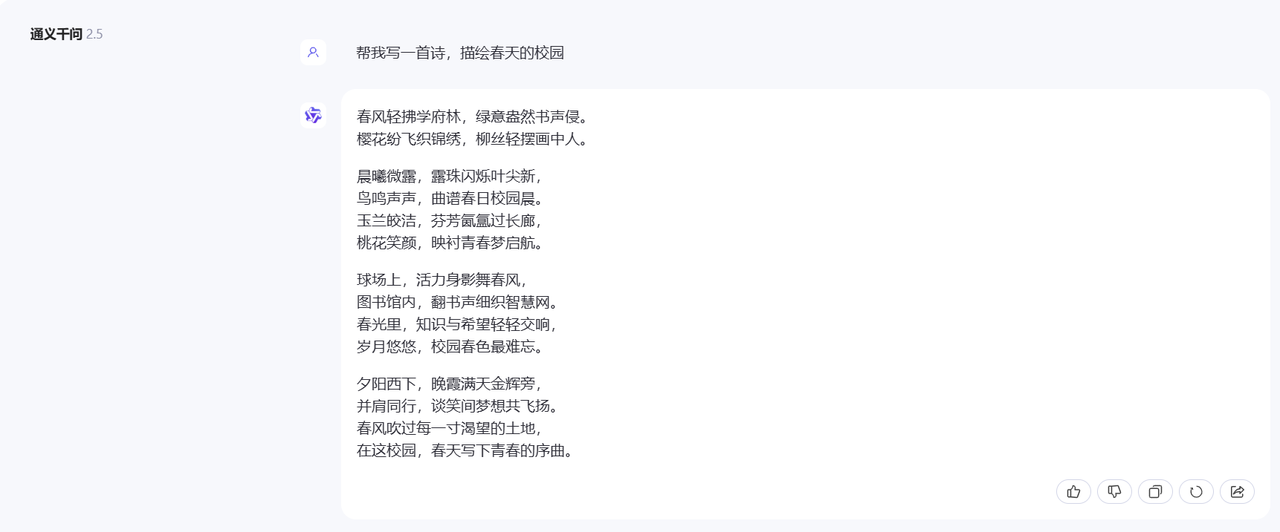
\includegraphics{images/Internet_10.png}
\end{marginfigure}

\subsection{AI绘画}
\begin{marginfigure}
    
\includegraphics{images/Internet_01.jpg}
\end{marginfigure}
曾经画家为了创作一幅画需要不断构思,不断修改,花费多少个日日夜夜才能得到一个满意的作品,然而如今人们只需要下达几个简单的文字指令,AI就能自动画出多张精致的作品。而在众多的AI绘画模型中,Stable diffusion无疑是现今使用的最为广泛,最广为认知的了。

Stable diffusion是一款由Stablility AI公司于2022年所开发的AI绘画生成模型。由于该模型操作简便,且生成速度快,平均只需要10到20秒即可获得一张精致的画作,一经推出就受到广大网友的喜爱。那么这款模型具体是怎么运作的呢?

具体地说,Stable diffusion用的是latent diffusion model(隐扩散模型)。这是一种文本到图像的深度学习模型,输入文本,模型即可输出相关的图像。它一共由三个模块组成,分别是(变分自动编码器)VAE,文本编码器和U-Net。输入文字描述,该模型通常可以分为下面几步运作:
1. 首先模型随机生成图像,变分自动编码器把该图像从像素空间压缩到更小维度的隐空间。
2. 对隐空间中的图片添加噪声,进行扩散过程。
3. 通过文本编码器将输入的描述语转换为去噪过程的条件。
4. 基于文本编码器得到的条件,U-Net会对图像进行去噪。
5. 最终使用变分自动编码器将图像从隐空间转换回像素空间,得到图像。
除了输入文字描述得到相应图像,通过把中间的文本编码器替换成图像+文本的编码器,模型还可以完成基于文字描述对输入图像进行修改的功能。

\subsection{AI作曲}
实际上,在SunoAI出现前,就有几款AI作曲的工具出现了,如网易天音,SongR等。不得不承认的是,这些较早期的AI作曲工具都是有作曲能力的,但相对于强人工智能,这些产品都只能算得上是“工具”的范畴,使用这些工具需要使用者具有一定的音乐的理论知识。然而作为一款针对音乐人的工具,它们的生成逻辑又显得过于机械化,没有给人们太多的自由度去创作。因此这些工具也就逐渐淡出了人们的视野。

SunoAI,作为音乐界的ChatGPT,在2024年的3月推出,一经推出便轰动了世界。和以前的AI作曲不一样,SunoAI只需要用户输入一句话的提示词,既可以在短短数秒内生成一首几分钟的完整的歌曲,从作词,作曲,到人声演唱一气呵成,大大降低了普通人创作音乐的门槛。已经习惯了各类“AI歌手翻唱”的听众和用户迅速拥抱了Suno,从《宫保鸡丁咏叹调》到《让我们荡起双桨》重金属,从英语、日语、俄语到普通话甚至是粤语,网友们自发上传的作品包罗万象,网易云音乐、QQ音乐等平台也迅速上线了SunoAI音乐专区,甚至还推出了定期更新的官方推荐歌单。

\section[网络安全与隐私保护]{网络安全与隐私保护:AI如何护航互联网安全}
当前的网络空间已经进入到了人工智能时代。人工智能对网络空间已经产生了深远的影响,是人工智能时代的安全问题呈现出了新的趋势。一是攻击者开始运用人工智能发起新型网络攻击;二是出现了针对人工系统本身的攻击或欺骗,从而导致人工智能模型出现一些分类或预测的错误;三是人工智能开始赋能安全,也即人工智能保障安全,是指利用人工智能来自动识别潜在的网络威胁的工具和技术。在这一章节,我们将讨论当前人工智能如何护航互联网安全。

\subsection{恶意代码智能分析检测}
近年来,网络空间面临严峻的安全威胁,其中,僵尸网络,木马,蠕虫攻击就是威胁的典型代表。恶意代码作为攻击的载体,会在互联网上进行传播,可以定向传输至被攻击的目标。被攻击目标若运行了这些恶意代码,会造成信息泄漏,数据损失,主机失陷等后果。在2017年,一种名为WannaCry的病毒在全球范围内引起了一阵风暴,这种病毒正式利用Windows系统的SMB服务相关漏洞进行传播,所有被病毒缠上的主机上的图片,文档,音频,视频,压缩包,可执行程序等文件会被加密,如果这些受害者不支付赎金,被加密的文件将会无法恢复。

恶意代码分析中引入机器学习方法的一般工作模块可以分为:数据预处理模块,特征工程模块,机器学习训练模块。根据不同的恶意代码的类型,会采取不同的预处理方法,然后再选择人工定义和自动提取相结合的特征工程方法,通过特征工程模块输出的特征向量作为机器学习训练模块的输入,进行有监督的学习,最后训练好的分类器可以应用于实际的恶意代码检测。

以PE二进制恶意代码为例,给出一个具体的技术方案。首先,在数据预处理模块中,将待检测的PE二进制格式可执行代码在虚拟机中运行,监控并记录所产生的系统API调用序列;然后,对获得API序列进行特征工程,其中可以用N-gram模型,word2vec模型等方法将API序列转换为特征向量,这样就完成了机器学习前的工作。将特征向量作为机器学习模型的输入,机器学习模型则可以有很多选择,具体模型性能需要结合具体的场景来分析,可以使用传统的机器学习分类器如决策树,支持向量机,XGBoost等,亦可以使用神经网络模型,如卷积神经网络等深度学习分类器。通过在大规模的有监督数据上进行学习,模型可以获得较好的检测恶意代码的能力。

\subsection{恶意网页识别}
由360安全中心发布的《2019年网络诈骗趋势研究报告》显示,2014到2019年,网络诈骗人均损失逐年增长。当前的诈骗网站已经不局限于通过钓鱼网站来盗取用户的隐私数据,虚拟信贷,网络赌博等新型诈骗网站层出不穷。随着互联网的飞速发展,诈骗网站的内容也在不断变化,行为越来越难以检测,发展态势日趋产业化。

针对恶意网页日益增长的趋势,当前很多浏览器如Google Chrome,Edge等都已经可以检测识别出恶意网页,在用户点击网站时,若浏览器检测出其恶意攻击行为,就会阻止用户进入网站,从而保护了用户的个人隐私和财产安全。而这样的技术基本都是基于人工智能技术的,下面我们以中国移动提出的一个基于人工智能的诈骗网站识别方案为例,具体说明人工智能是如何为互联网安全保驾护航的。

诈骗网站识别方案的整体流程可以分为以下5个部分:
1. 收集活跃域名
2. 域名发现与拓展
3. 域名取证分析
4. 人工审核
5. 域名封堵
首先,从互联网数据中获取活跃的域名,利用人工智能模型来检测分析出潜在的诈骗域名,然后通过爬虫软件对潜在诈骗域名进行内容的爬取和分析,筛选出高度疑似诈骗网站的网站,交由人工进行审核,最后对于可以确定的诈骗域名进行封堵操作。这套恶意诈骗网站识别方案在2019年上线应用,每天会分析超过200亿条上网日志,垃圾短彩信,用户举报,每月能检测出诈骗网站超4万个,组断了2004.9亿次的诈骗网站访问,有效地保护了用户的个人隐私和财产安全。

第一步的域名发现会对网络中存在访问行为的域名进行搜集,并将这些域名信息作为全网的活跃域名全集。活跃域名全集的数据来源包括垃圾短彩信中的域名信息,用户投诉举报数据中的域名信息,以及用户的上网日志等。进而通过消息智能分类,域名智能分类,注册备案分析,流量日志分析,从收集得到的活跃域名全集发现潜在的诈骗域名。
域名拓展
活跃域名全集中的域名发现模块能够识别出可能的诈骗网站,但这意味着域名识别的时机已经晚于用户的访问,形成了事后识别的情况。然而,通过引入域名拓展模块,可以有效地填补域名发现模块的缺陷,甚至在现实网络中用户访问行为被监测到之前,就能发现并识别出潜在的诈骗网站,从而实现对诈骗网站的事前管理。
域名拓展模块具有根据已知欺诈域名信息进行进一步挖掘和发现的功能,可以找到更多与已知欺诈域名有关联的潜在欺诈域名,它由网站外链拓展、备案信息拓展、域名数字拓展和相似风格拓展四个子模块构成。
网站外链拓展:一些欺诈网站,如赌博类和色情类网站,通常会通过友情链接或广告的方式互相链接,方便用户在网站之间进行跳转。网站外链拓展模块利用这一特点,对已知欺诈网站中的外链信息进行迭代爬取,重点抓取欺诈网站中的友情链接和广告链接,以发现更多的潜在欺诈域名。
注册信息拓展:欺诈网站的创建者通常会批量注册大量的域名,我们可以利用域名注册信息的属性关联性来实现域名的拓展。注册信息拓展模块通过已知欺诈域名的备案联系人信息,反查该联系人注册的其他域名信息,将这些域名作为潜在欺诈域名。
域名数字拓展:在赌博类欺诈网站的域名中,通常会包含大量的数字。域名数字拓展模块对已知欺诈域名中的数字进行尝试性改变,以拓展域名,然后通过爬虫爬取并验证可访问性,从而获取潜在的欺诈域名。
相似风格拓展:欺诈网站的创建者在选择域名时,往往会倾向于特定的域名风格。相似风格拓展模块利用人工智能技术,学习已知欺诈域名的组成风格,然后利用人工智能的创作能力,生成更多与已知欺诈域名风格相似的潜在欺诈域名。由于人工智能技术生成的域名可能并不真实存在,因此需要结合爬虫技术,排除掉无法访问的潜在欺诈域名。
域名取证分析
内容分析取证模块对潜在诈骗域名的网站内容进行全面评估,从而找出高度疑似的诈骗网站,并将相关爬取内容作为判断依据提交给人工审核。在爬取网站的过程中,需要收集网站的文本信息、源码信息、图片信息,同时需要对网站的最终展示效果进行截图。收集到网站内容信息后,内容分析取证模块从文本、源码、图片、视觉等多个角度对网站进行诈骗特征分析,并将高度疑似的诈骗网站提交至人工审核平台。
人工审核
尽管当前的人工智能检测恶意诈骗网站的准确率已经很高,但是仍然会出现部分识别错误的情况,如把没有攻击行为的网站识别为恶意诈骗网站。因此我们还需要人工审核来确定网站是否为诈骗网站。对于恶意诈骗网站,人工审核平台会向域名封堵模块下达封堵指令
域名封堵
为了能够有效防止用户访问诈骗网址,域名封堵模块将判定为诈骗域名加入拦截名单,当有用户请求 拦截名单中的域名时,则中断用户请求,并向用户请求重定向到安全提示页面。